\documentclass[
    10pt,
    aspectratio=169,
    xcolor={dvipsnames},
    spanish,
    % handout,
    % notes=only,
    % notes,
    ]{beamer}

% BEAMER SETTINGS
\setbeamerfont{section in toc}{size=\normalsize, shape=\bfseries}
\mode<presentation>{
    \usetheme{Antibes}
    \setbeamercovered{transparent}
    \usecolortheme{rose}
    \setbeamertemplate{navigation symbols}{}
    }
\useoutertheme{infolines}

% PACKAGES
% \usepackage[spanish]{babel}  % uncomment for Spanish support
\usepackage{tikz,pgfplots}
\pgfplotsset{compat=1.13}
\usetikzlibrary{calc}
\usepackage{subcaption}
\usepackage{graphicx}
\graphicspath{{figures}}
\usepackage{booktabs}
\usepackage{upgreek}
\usepackage{commath}
\usepackage{amsmath,amsthm,amssymb,mathtools,mathrsfs}
\usepackage{cancel}
\usepackage{fontawesome5}
\usepackage{enumerate}
\usepackage{tensor}
\usepackage[font=footnotesize]{caption}
\usepackage{wasysym}

\usepackage[skins,theorems]{tcolorbox}
\tcbset{
    highlight math style={
        enhanced,
        coltext=black,
        colframe=black,
        colback=lightgray,
        arc=0pt,
        boxrule=.5pt
        }
}

% REFERENCES AND OTHERS
\usepackage{aas_macros}
\usepackage{natbib}
\bibpunct{(}{)}{;}{a}{}{,}

\usepackage{siunitx}
\sisetup{
    range-phrase=\text{--},
    range-units=single,
    separate-uncertainty=true,
    print-unity-mantissa=false
    }
\DeclareSIUnit{\gauss}{G}
\DeclareSIUnit{\jansky}{Jy}
\renewcommand{\figurename}{Fig.}

\usepackage{hyperref}
\hypersetup{
    % bookmarks=true,
    unicode=true,
    pdftoolbar=true,
    pdfmenubar=true,
    pdffitwindow=false,
    pdfstartview={FitH},
    pdftitle={ISI-Free Linear Combination Pulses with Better Performanc},
    pdfauthor={Erik Saez A.},
    pdfcreator={Erik Saez A.},
    pdfnewwindow=true,
    colorlinks=true,
    linkcolor=RoyalBlue,
    citecolor=RoyalBlue,
    urlcolor=RoyalBlue
    }

\title[Auxiliar \#4]{\bfseries Auxiliar \#4}
\subtitle{[EL3204] Controlabilidad, observabilidad y control por retroalimentación de estados}
\author[Erik Saez A.]{Erik Saez A.}
\institute[UChile]{Department of Electrical Engineering \\ Universidad de Chile}

\date{\today}

\begin{document}

\begin{frame}
  \titlepage
  \centering
  \faIcon{envelope} \href{mailto:erik.saez@ug.uchile.cl}{erik.saez@ug.uchile.cl} \hspace{.2cm}
  \faIcon{github} \href{https://github.com/ErikSaezA/Auxiliares}{ErikSaezA/Auxiliares} \hspace{.2cm}
  \faIcon{discord} \href{https://discord.gg/ubthV3cudQ}{Discord}
\end{frame}

\begin{frame}
  \frametitle{Contenidos}
  \centering
  \begin{columns}
    \begin{column}{0.4\textwidth}
      \tableofcontents
    \end{column}
    \begin{column}{0.5\textwidth}
      \begin{figure}
        \centering
        
\includegraphics[width=\textwidth]{fcfm_die}
        \caption{Facultad de Ciencias Físicas y Matemáticas , Universidad de Chile.}
      \end{figure}
    \end{column}
  \end{columns}  
\end{frame}
%%%%%%%%%%%%%%%%%%%%%%%%%%%%%%%%%%%%%%%%%%
\section{Estabilidad BIBS y BIBO}
%%%%%%%%%%%%%%%%%%%%%%%%
\begin{frame}{Estabilidad: BIBS y BIBO}
\footnotesize
\begin{columns}[T]
  \begin{column}{0.56\textwidth}
    \begin{block}{¿Qué miden?}
      \begin{itemize}\itemsep2pt
        \item \textbf{BIBS} (bounded–input bounded–state): con entradas y C.I. acotadas, el \emph{estado} permanece acotado (estabilidad interna).
        \item \textbf{BIBO} (bounded–input bounded–output): con entradas acotadas, la \emph{salida} permanece acotada (estabilidad externa).
      \end{itemize}
    \end{block}
    \begin{block}{Criterios prácticos (LTI)}
      \begin{itemize}\itemsep2pt
        \item \textbf{BIBS}: continuo $\Rightarrow \mathrm{Re}\{\lambda_i(A)\}<0$;\; discreto $\Rightarrow |\lambda_i(A)|<1$.
        \item \textbf{BIBO} (SISO): continuo $\int_0^{\infty}|h(t)|\,dt<\infty$ $\Leftrightarrow$ polos de $H(s)$ en $\mathrm{Re}\,s<0$;\\
        discreto $\sum_{k\ge 0}|h[k]|<\infty$ $\Leftrightarrow$ polos de $H(z)$ dentro del disco unidad.
      \end{itemize}
    \end{block}
  \end{column}
  \begin{column}{0.42\textwidth}
    \begin{block}{Relación y matices}
      \begin{itemize}\itemsep2pt
        \item \textbf{BIBS $\Rightarrow$ BIBO}. Si la realización es \emph{mínima} (controlable y observable), \textbf{BIBS $\Leftrightarrow$ BIBO}.
        \item La BIBO depende de $H(\cdot)$ (por $C,D$); la BIBS depende solo de $A$.
        \item En la \emph{frontera} (autovalores en eje imaginario o $|z|{=}1$) puede haber estabilidad \emph{marginal} (no BIBO si hay polos repetidos).
      \end{itemize}
    \end{block}
  \end{column}
\end{columns}
\end{frame}

\section{Controlabilidad y observabilidad}
%%%%%%%%%%%%%%%%%%%%%%%%
\begin{frame}{Controlabilidad y observabilidad: qué, cómo y para qué}
\footnotesize
\begin{columns}[T]
  \begin{column}{0.52\textwidth}
    \begin{block}{¿Qué miden?}
  	\textbf{Controlabilidad}: alcanzar cualquier estado con entradas adecuadas.\\
  	\textbf{Observabilidad}: reconstruir el estado a partir de $u(\cdot)$ y $y(\cdot)$.
    \end{block}
    \begin{block}{Kalman (criterio de rango)}
      \begin{align}
        \mathcal C &= [\,B\;AB\;\cdots\;A^{n-1}B\,], & \operatorname{rank}(\mathcal C){=}n &\iff \text{controlable},\\
        \mathcal O &= \begin{bmatrix} C\\ CA\\ \vdots\\ CA^{n-1}\end{bmatrix}, & \operatorname{rank}(\mathcal O){=}n &\iff \text{observable}.
      \end{align}
    \end{block}
  \end{column}
  \begin{column}{0.47\textwidth}
    \begin{block}{Gramianos (continuo, $A$ Hurwitz)}
      \begin{align}
        A W_c + W_c A^\top + B B^\top &= 0, & W_c\succ 0 &\iff \text{controlable},\\
        A^\top W_o + W_o A + C^\top C &= 0, & W_o\succ 0 &\iff \text{observable}.
      \end{align}
    \end{block}
    \begin{block}{Implicancias prácticas}
      \begin{itemize}\itemsep2pt
        \item \textbf{Realización mínima}: controlable y observable $\Rightarrow$ sin modos ocultos.
        \item \textbf{Ubicación de polos} (REN(C)): factible $\iff$ controlable; \textbf{observador} (RENC): factible $\iff$ observable.
        \item Modos incontrolables no pueden estabilizarse; modos inobservables no aparecen en $y$.
      \end{itemize}
    \end{block}
  \end{column}
\end{columns}
\end{frame}
%------------------------------
\section{Control por retroalimentación de estados}
%%%%%%%%%%%%%%%%%%%%%%%%
\begin{frame}{Control por retroalimentación de estados}
\footnotesize
\begin{block}{¿Qué es y para qué sirve?}
  El \textbf{control por retroalimentación} (o \emph{feedback}) permite determinar qué debería ocurrir en base al estado actual del sistema. Se utiliza el estado actual para modificar la entrada al sistema, considerándola dentro de $u(t)$:
  \[ u = -Kx + r \]
  donde $K$ es la matriz de ganancia de retroalimentación y $r$ es la señal de referencia.
\end{block}

\begin{columns}
  \begin{column}{0.52\textwidth}
    \begin{block}{Sistema en lazo cerrado}
      Con la retroalimentación $u = -Kx + r$:
      \begin{align}
        \dot{x} &= Ax + Bu = (A - BK)x + Br \\
        \tilde{A} &:= A - BK
      \end{align}
      La matriz de transición de estados es:
      \[ \Phi(t_0, t) = e^{\tilde{A}(t-t_0)} \]
      Los autovalores de $\tilde{A}$ dominan la respuesta del sistema.
    \end{block}
  \end{column}
  \begin{column}{0.46\textwidth}
    \begin{block}{Teorema fundamental}
      \textbf{Teorema:} Si $(A,B)$ es controlable, entonces $\exists K$ tal que $E = A - BK$ tiene espectro arbitrario.
      
      Esto significa que podemos ubicar los polos del sistema en lazo cerrado en cualquier posición deseada del plano complejo.
    \end{block}
  \end{column}
\end{columns}
\end{frame}
%------------------------------
\begin{frame}{Diagrama de bloques: Control por retroalimentación de estados}
\footnotesize
\begin{columns}
  \begin{column}{0.58\textwidth}
    \begin{figure}
      \centering
      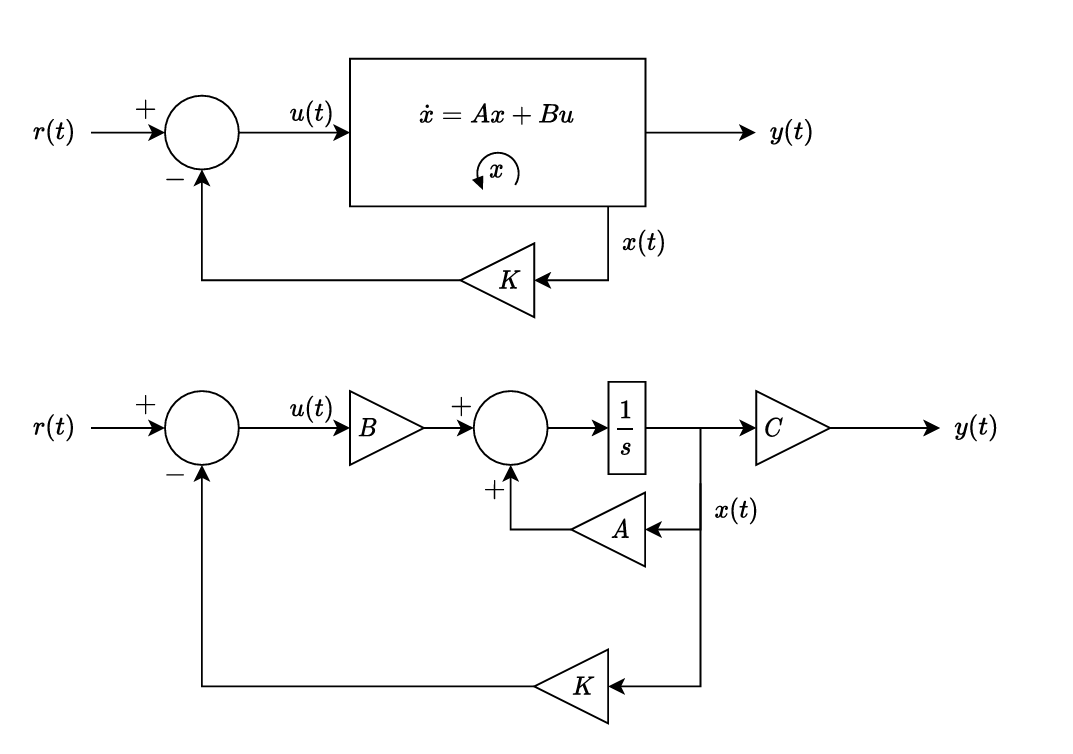
\includegraphics[width=\textwidth]{Figura_5.png}
      \caption{Representaciones del sistema con retroalimentación de estados.}
    \end{figure}
  \end{column}
  \begin{column}{0.40\textwidth}
    \begin{block}{Descripción del diagrama}
      \textbf{Diagrama superior:} Representación compacta
      \begin{itemize}\itemsep1pt
        \item $r(t)$: señal de referencia
        \item $u(t) = -Kx(t) + r(t)$: ley de control
        \item $K$: matriz de ganancia de retroalimentación
        \item El estado $x(t)$ se retroalimenta para formar la entrada de control
      \end{itemize}
      
      \textbf{Diagrama inferior:} Representación detallada
      \begin{itemize}\itemsep1pt
        \item Muestra explícitamente las matrices $A$, $B$, $C$
        \item Integrador $\frac{1}{s}$ para obtener $x(t)$ desde $\dot{x}(t)$
        \item Retroalimentación completa del vector de estados
      \end{itemize}
    \end{block}
  \end{column}
\end{columns}
\end{frame}
%%%%%%%%%%%%%%%%%%%%%%%%
\section{Pregunta 1}
\begin{frame}{Pregunta \#1}
  \footnotesize
\begin{block}{Enunciado Pregunta \#1}
 Considere el sistema en tiempo continuo dado por
  \begin{equation}
      \ddot y(t) - 2\dot y(t) - 8 y(t) = 3\dot u(t) + 3 u(t),
      \label{eq:plant}
  \end{equation}
  donde $u(t)$ es la entrada y $y(t)$ la salida.

  \begin{enumerate}
    \item Obtenga la función de transferencia $G(s)=\dfrac{Y(s)}{U(s)}$ del sistema (condiciones iniciales nulas).
    \item A partir de $G(s)$, proponga una representación en espacio de estados $(\dot x = Ax + Bu,\; y = Cx + Du)$ en forma controlable.
    \item Determine si el sistema es controlable y observable. Justifique mediante los rangos de las matrices de controlabilidad y observabilidad.
    \item Diseñe un controlador por realimentación de estados $u = -Kx + r$ que ubique los polos a lazo cerrado en $s=-5$ y $s=-3$. Indique el vector $K$.
    \item Suponga ahora que sólo se mide la salida $y(t)$ y no el estado completo. Diseñe un compensador dinámico (controlador con observador de estado) que mantenga los polos de lazo cerrado en $-5$ y $-3$. Indique los polos del observador y el vector de ganancias $L$.
  \end{enumerate}
\end{block}
\end{frame}
%%%%%%%%%%%%%%%%%%%%%%
\section{Pregunta 2}
\begin{frame}{Pregunta \#2}
\footnotesize
Considere un motor eléctrico DC que impulsa un carrito, como se muestra en la figura.
  \begin{center}
    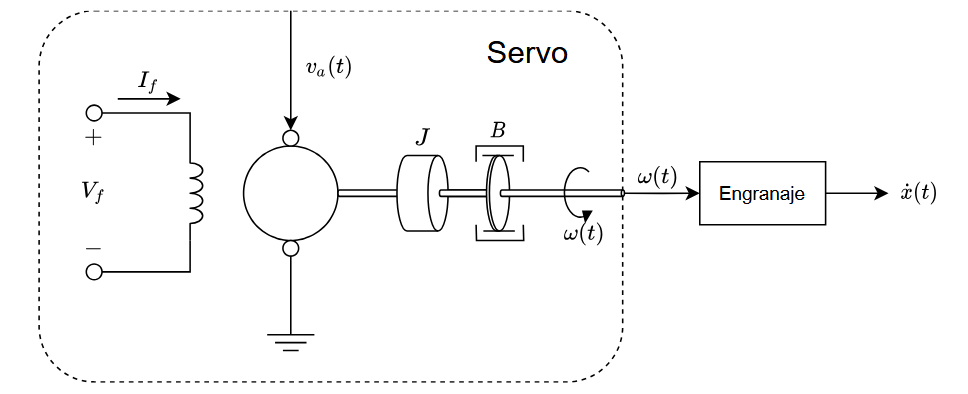
\includegraphics[width=.65\textwidth]{Figura_6.png}
  \end{center}
  Suponga que los parámetros del sistema son:
  \begin{align}
     k_m &= 1\;\text{Nm/A}, & k_e &= 1\;\text{Vs}, & R_a &= 0.01\,\Omega, \\
     L_a &= 1\,\text{H}, & J &= 0.1\,\text{kgm}^2, & B &= 0.2\,\text{Nms}, \\
     k_g &= 0.01\,\text{m/rad}. & &
  \end{align}
\end{frame}
\begin{frame}{Pregunta \#2 (continuación)}
  \begin{block}{Enunciado Pregunta \#2 (continuación)}
  \begin{enumerate}
    \item Formule un modelo dinámico del sistema en variables de estado, indicando claramente las hipótesis simplificatorias.
    \item Encuentre la función de transferencia desde el voltaje de armadura $v_a(t)$ hasta la velocidad lineal $\dot z(t)$ del carrito.
    \item Determine si el sistema es estable (según los polos de la función de transferencia / matriz $A$).
    \item Obtenga la respuesta al impulso de la salida $\dot z(t)$.
    \item Exprese la respuesta del sistema en un tiempo arbitrario $t$ para condiciones iniciales y entrada arbitraria.
    \item Determine si el sistema es completamente controlable y observable.
    \item En caso de ser observable, diseñe un observador cuyos polos se ubiquen en $-10$ y $-5$.
  \end{enumerate}
\end{block}
\end{frame}

%%%%%%%%%%%%%%%%%%%%%%


\end{document}
